Il \textit{Data Analyzer} si occupa dell'analisi dei dati raccolti dal \textit{Data Collector}, al fine di generale allarmi che saranno poi visibili agli utenti. Come per il \textit{Data Collector}, si è scelto di implementare questo componente come un applicativo Python, che verrà poi distribuito su un Raspberry Pi per l'esecuzione. Si è scelto questo linguaggi di programmazione poiché sono presenti molte librerie per effettuare analisi dei dati, che verranno sfruttate per la generazione di allarmi. In particolare, si è scelto di implementare la generazione di allarmi per pericolo di nebbia o brina e di maltempo imminente. Nella figura \ref{fig:DAFlowChart} è rappresentato il flusso di esecuzione del Data Analyzer. All'avvio dell'applicazione, vengono inizializzate alcune strutture dati necessarie agli algoritmi, presentati di seguito, per l'analisi dei dati. Successivamente, viene eseguito un tentativo di connessione al DB, seguendo una strategia uguale a quella utilizzata nel Data Collector. Se la connessione è stabilita con successo, vengono recuperati dal DB i codici identificativi delle stazioni meteorologiche e salvati. Essi saranno utilizzati successivamente per recuperare i dati necessari agli algoritmi di generazione degli allarmi. Successivamente, viene avviato un thread per ogni zona, che si occuperà della generazione delle allerte maltempo, analizzando i dati relativi alla pressione atmosferica. Inoltre, vengono avviati i thread che si occupano di analizzare i dati al fine di generare allarmi di nebbia e brina. Viene attesa la terminazione di tutti i thread avviati e, al termine, viene chiusa la connessione con il database. Il ciclo viene ripetuto ogni 5 minuti.

\begin{figure}[h!]
	\centering
	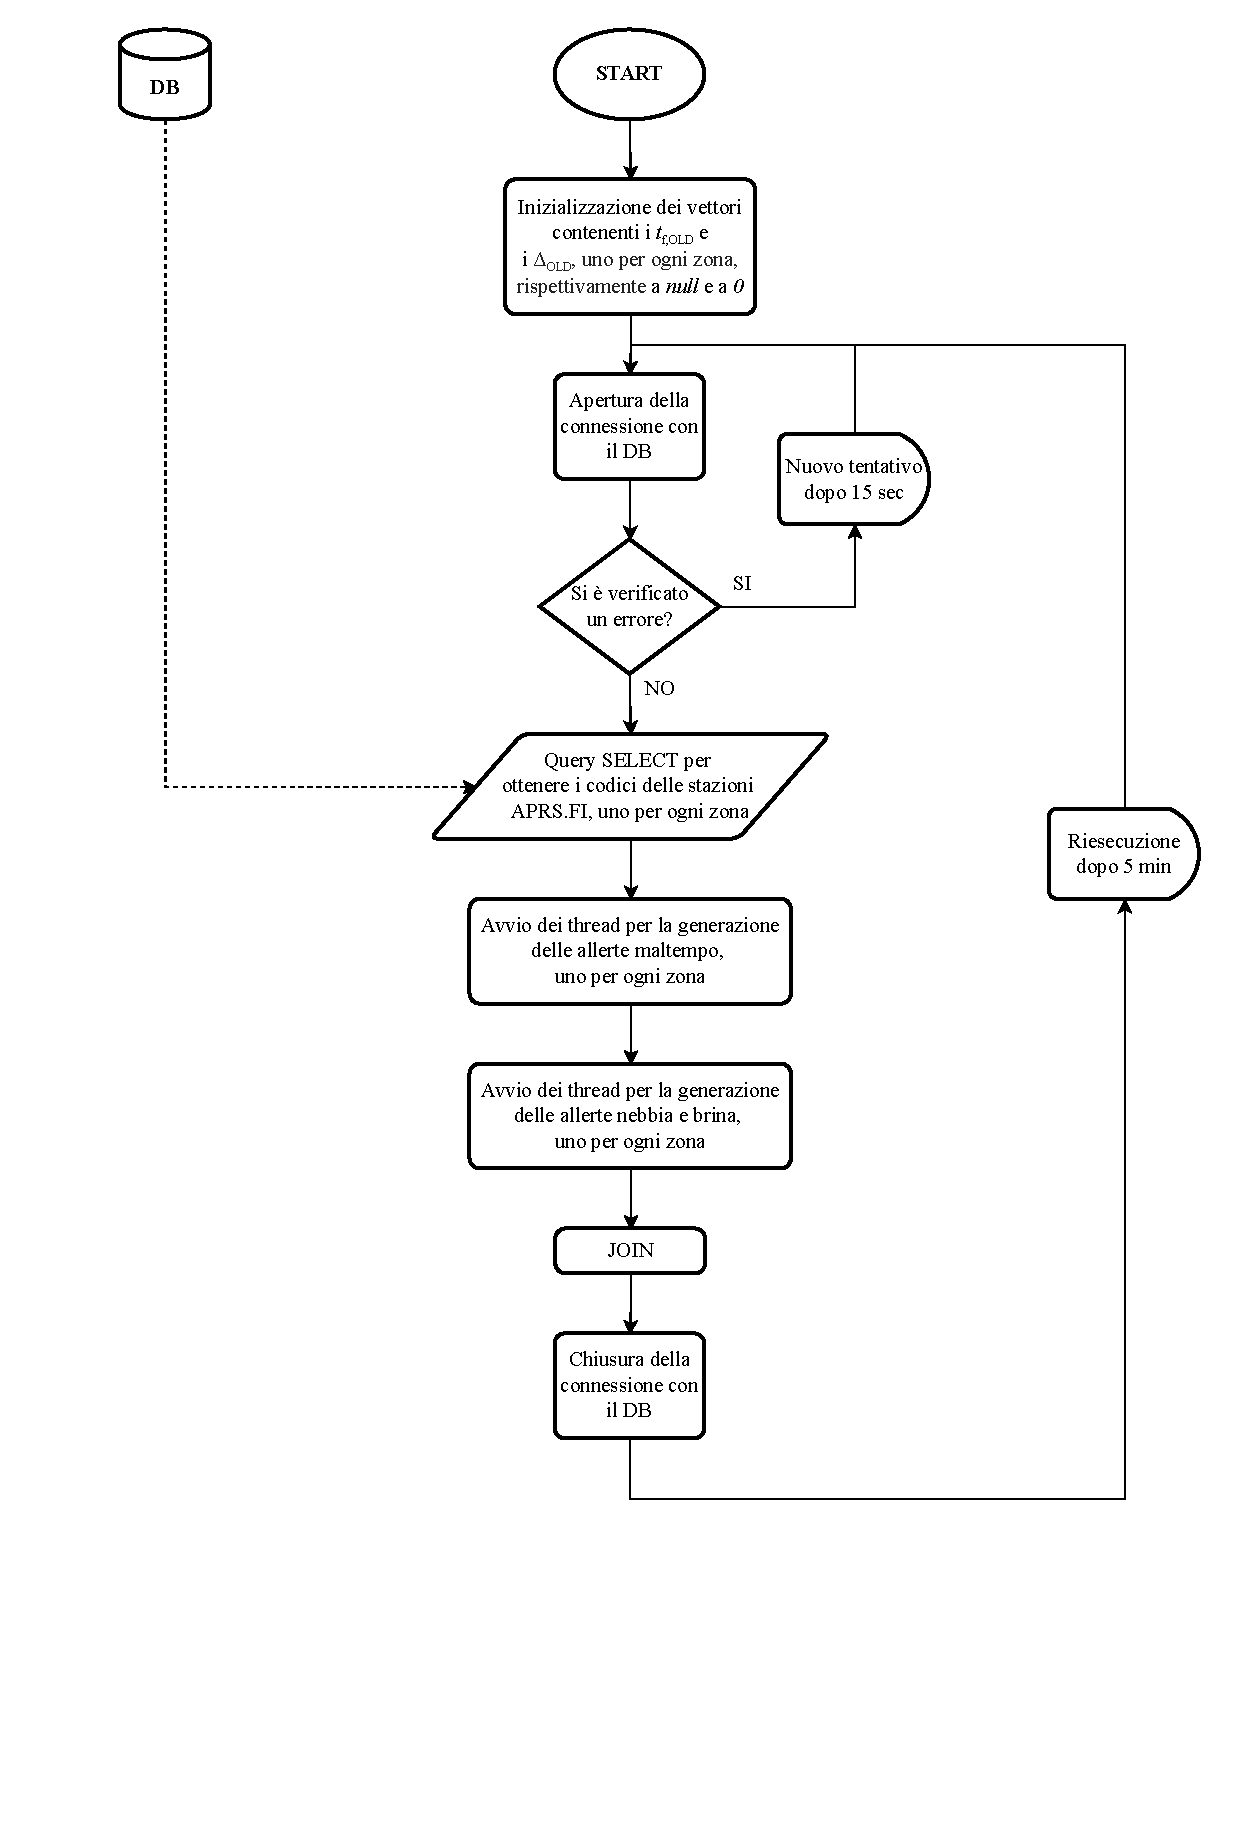
\includegraphics[width=1\linewidth]{./Iterazione 3/OtherFiles/FC - data analyzer}
	\caption{Diagramma di flusso di esecuzione del componente Data Analyzer.}
	\label{fig:DAFlowChart}
\end{figure}

\paragraph{Allerte maltempo}
\todo{da inserire}
\paragraph{Allerte brina/nebbia}
\todo{da inserire}